\documentclass[handout]{beamer}

\usepackage[T2A]{fontenc}
\usepackage[cp1251]{inputenc}
\usepackage[english]{babel}
\usepackage{amssymb,amsmath,amsthm,amsfonts}
\usepackage{graphicx}
\defbeamertemplate*{footline}{Warsaw} {%
\leavevmode%
\hbox{%
\begin{beamercolorbox}[wd=.58\paperwidth,ht=2.5ex,dp=1.125ex,leftskip=.3cm,rightskip=.3cm]{author in head/foot}%
\insertframenumber{}%
\hfill\insertshortauthor{}
\end{beamercolorbox}%
%%\begin{beamercolorbox}[wd=.42\paperwidth,ht=2.5ex,dp=1.125ex,leftskip=.2cm,rightskip=.2cm]{title in head/foot}%
%%\usebeamerfont{title in head/foot}
%%\insertshorttitle{Efficient First Order Inductive Learner on Spark}
%%\end{beamercolorbox}
}%
\vskip0pt%
}
\title{\qquad Distributed Big Data Analytics\qquad\qquad\qquad\\ Efficient First Order Inductive Learner on Spark}
\author{ Georgiy Shurkhovetskyy, Eskender Haziiev \\ Supervisors: Hajira Jabeen, Gezim Sejdiu}
\institute{University of Bonn, 2017}

\date{}



\begin{document}

%------------------------------------------------ 1
\begin{frame}
%\transdissolve[duration=0.4]
  \titlepage
\end{frame}







%%------------------------------------------------------------------- 2
\begin{frame}{Problem Statement}
\footnotesize

\textbf{Definition 1}. A literal $L$ may be predicate $P$ or
 $\neg{P}$.

\textbf{Definition 2}. A clause body is a conjunction of literals.

\textbf{Definition 3}. A clause head is predicate.

\textbf{Definition 4}. A Horn clause consists of a head and a
 body:
\begin{equation}\label{eq0}
P\leftarrow L_1,L_2,..., L_n .
\end{equation}
\textbf{Definition 5}. A learning rule for predicate $P$ is
 a collection of Horn clauses each with head $P$.

The predicates can be defined \emph{extensionally} as a list of
tuples for which the predicate is true, or \emph{intensionally} as
a set of Horn clauses.


\textbf{Definition 6}. $k$-tuple $<a_1, a_2, \ldots, a_k>$ is a
finite sequence of $k$ constants.

\textbf{Definition 7}. A tuple satisfies a learning rule if it
satisfies one of the Horn clauses of this rule.

For every relation a set of the $\oplus$tuples  which
 belong to this relation is given.

For a target relation a set of $\oplus$tuples is also given. A set
of the $\ominus$tuples not belonging to the target relation may be
given. The statement is introduced: if some tuple is not included
in set $\oplus$tuples then it is $\ominus$tuple.

\textcolor[rgb]{0.00,0.00,1.00}{\textbf{Problem statement:}} Using
Spark framework realize FOIL to find a learning rule as a set of
Horn clauses for the target relation that consistent with given
positive examples and not cover any given negative examples.
\end{frame}

%%------------------------------------------------------------------------------------------ 3
\begin{frame}{Approach}
Foil algorithm is realized using Scala in Spark framework.
\begin{figure}[h!]\centering
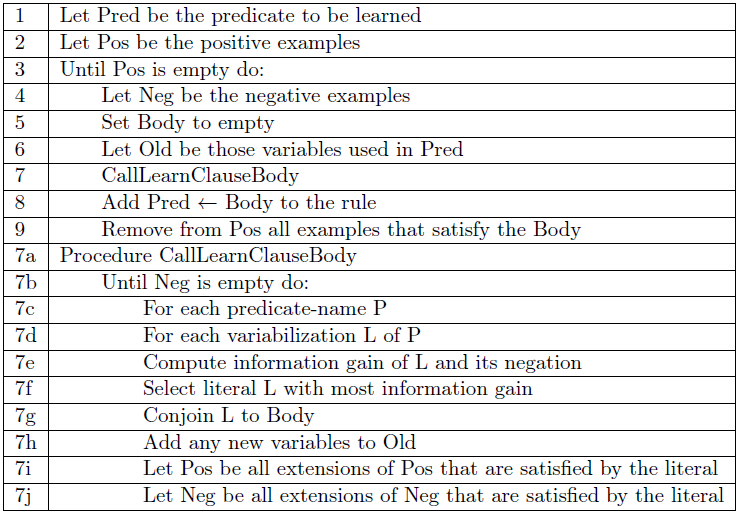
\includegraphics[scale =0.42]{approach.png}
\end{figure}
\vspace{-6pt} \footnotesize{To select literal with greatest
positive gain:}
\begin{equation}\label{eq4}
gain (L_{i})=n_i^{\oplus\oplus} \cdot (I(T_i)-I(T_{i+1})),\quad
I(T_i)=-\log_2 (n_i^\oplus/(n_i^\oplus+n_i^\ominus)),
\end{equation}
$n_i^\oplus$ --- a number of $\oplus$tuples in $T_i$,
$n_i^\ominus$ --- a number of $\ominus$tuples in $T_i$,\\
$\!\!\!\!n_i^{\oplus\oplus}$ --- a number of the $\oplus$tuples in
$T_i$ represented by one or more tuples in $T_{i+1}$.
\end{frame}


%%------------------------------------------------------------------------------------------ 4
\begin{frame}{Implementation}
\begin{figure}[t]\centering
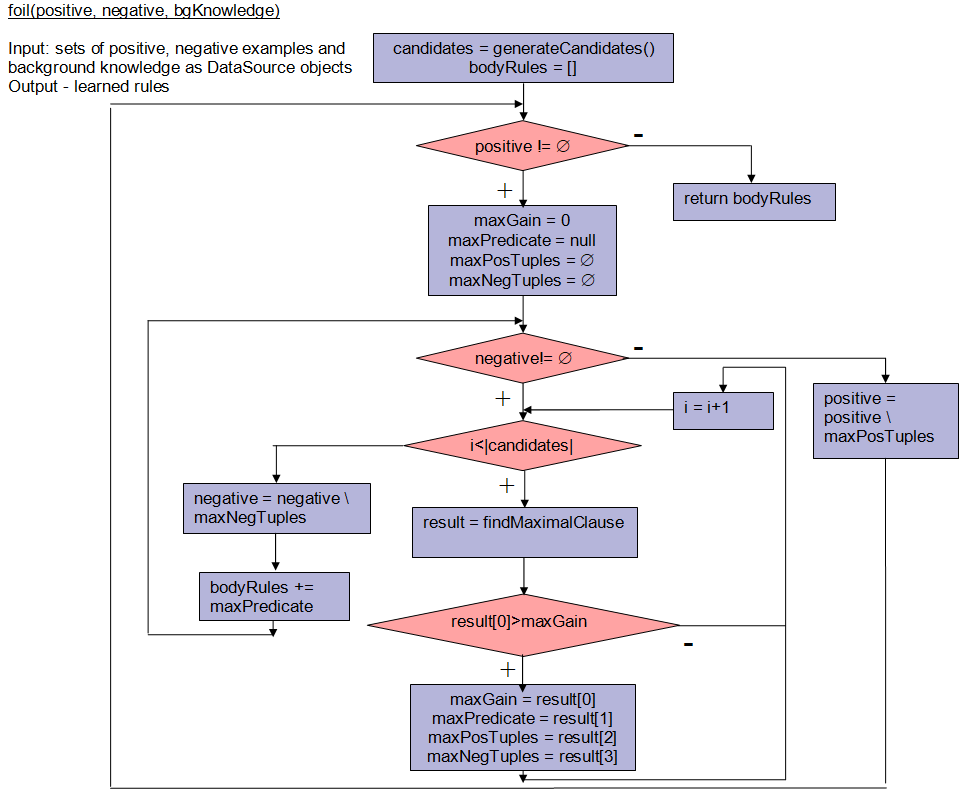
\includegraphics[scale =0.39]{shema.png}
\end{figure}
\end{frame}

%%------------------------------------------------------------------------------------------ 5
\begin{frame}{Evaluation}
\vspace{-2pt}
\textcolor[rgb]{0.00,0.00,1.00}{\underline{Evaluation metrics:}}  $\rho_k(A_1,A_2)=|n_k(A_1)-n_k(A_2)|$, $k=1,2,3$.

\footnotesize{Indicators:}
$n_1(A)=\frac{n^\oplus_{\textrm{covered}}(A)}{n^\oplus_{\textrm{given}}}$, $n_2(A)=\frac{n^\ominus_{\textrm{covered}}(A)}{n^\ominus_{\textrm{given}}}$, $n_3(A)=\textrm{runtime}(A)$.

\vspace{2pt}
\textcolor[rgb]{0.00,0.00,1.00}{Experiment 1.} (a), \underline{results:} $daughter(X_1,X_2) \leftarrow female(X_1) parent(X_2,X_1)$;\\ covered $\oplus$ examples: (Emily, Tom), (Mary, Ann); covered $\ominus$ examples: $\emptyset$.

\textcolor[rgb]{0.00,0.00,1.00}{Experiment 2.} (b), \underline{results:} $daughter(X_1,X_2) \leftarrow female(X_1) parent(X_2,X_1)$;\\ covered $\oplus$ examples: (Opra, Ann), (Kate, Ann), (Lina, Kate), (Gail, Hovard); covered $\ominus$ examples: $\emptyset$.

\textcolor[rgb]{0.00,0.00,1.00}{Experiment 3.} (b), \underline{results:} $son(X_1,X_2) \leftarrow male(X_1) parent(X_2,X_1)$;\\ covered $\oplus$ examples: (Ryan, Uve), (Bill, Opra), (Hovard, Ann), (Nick, Kate), (Uve, Ann), (Tom, Uve); covered $\ominus$ examples: $\emptyset$.
\vspace{-8pt}
\begin{figure}[h!] \centering
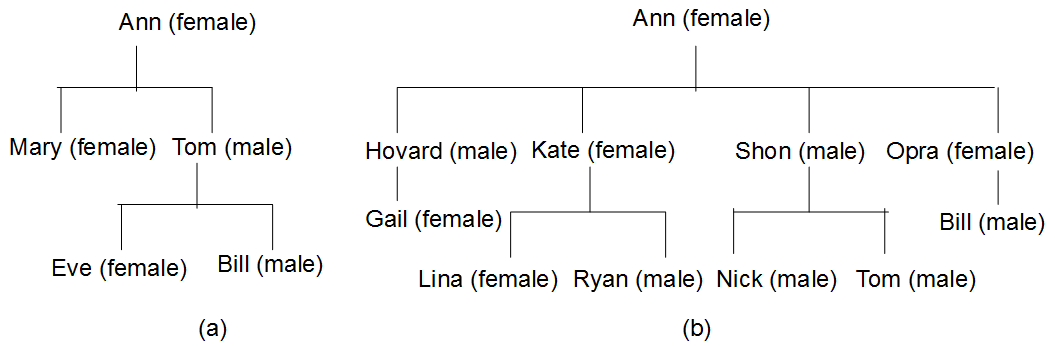
\includegraphics[scale =0.28]{tree_ds.png}
\end{figure}
\vspace{-10pt}
\begin{figure}[h!] \centering
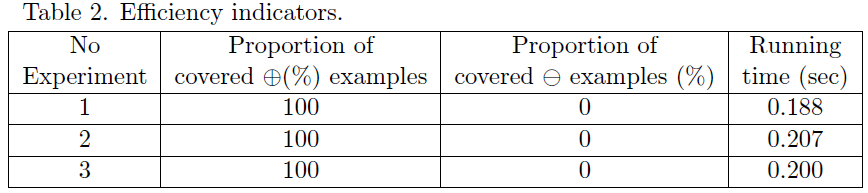
\includegraphics[scale =0.3]{Table2.png}
\end{figure}
\end{frame}

%%------------------------------------------------------------------------------------------ 6
\begin{frame}{Conclusion and future work}
\footnotesize \textcolor[rgb]{0.00,0.00,1.00}{Results of presented
project are:}

1. In Spark framework Foil algorithm is realized:

\qquad (i) the developed application gets the input data in
extensionally form (i.e. consists of names and $\oplus$ and
$\ominus$ tuples for target predicate, and names and $\oplus$
tuples for background predicates;)

\qquad (ii) the results are obtained  both in intensionally form
(i.e. as Horn clause for the target relation that consistent with
given $\oplus$tuples and not cover any given $\ominus$tuples) and
 extensionally form.

2. To evaluate developed application the metrics based on three
efficiency indicators are introduced.

3. three experiments were performed and on this base developed
application is evaluated as having sufficient efficiency.


\vspace {12pt}


\textcolor[rgb]{0.00,0.00,1.00}{The future steps to developed
application may be:}

1. Carrying out experiments with a more complex data structure,
for example, when a tree node is described by a large number of
predicates;

2. Evaluation of the application efficiency compared to other
implementations of the Foil algorithm.
\end{frame}

%%------------------------------------------------------------------------------------------ 7
\begin{frame}{Lesson learned}

Besides the detailed study of the FOIL algorithm

we also consider as the results of this project the following:

\vspace {12pt}

1. The extension of our skills on  applications development using
the Spark framework and the Scala programming language;

2. The receive of the skills in evaluation of an applications
effectiveness, including an experience in selection and drawing up
of the training data.

3. The extension of our experience on writing of the reports and
project drafting.

\end{frame}

%%------------------------------------------------------------------------------------------ 7
\begin{frame}{References}
\textcolor[rgb]{0.00,0.00,1.00}{[1]} T. Horvath. Learning in logic V. In Learning from Non-Standard Data, WS 2016/17.
University of Bonn, Fraunhofer IAIS, Sankt Augustin, Germany, 2016.

\textcolor[rgb]{0.00,0.00,1.00}{[2]} S. Muggleton and L. De Raedt. Inductive logic programming: Theory and methods.
The Journal of Logic Programming, 19(20):629�679, 1994.

\textcolor[rgb]{0.00,0.00,1.00}{[3]} M. Pazzani and D. Kibler. The utility of knowledge in inductive learning. Machine
Learning, 9(1):57�94, 1992.

\textcolor[rgb]{0.00,0.00,1.00}{[4]} J.R. Quinlan. Learning logical definitions from relations. Machine Learning, (5):239�266,
1990.

\textcolor[rgb]{0.00,0.00,1.00}{[5]} J.R. Quinlan and R.M. Cameron-Jones. Foil: A midterm report. In Machine Learning:
ECML-93, pages 3�20. Springer-Verlag, Berlin, Heidelberg, 1993.

\textcolor[rgb]{0.00,0.00,1.00}{[6]} J.R. Quinlan and R.M. Cameron-Jones. Induction of logic programs: Foil and related
systems. New Generation Computing, 13(3):287�312, 1995.
\end{frame}

\end{document}
